\section{VPC \& Networking}\label{sec:vpc-networking}

\subsection{EIP}\label{subsec:eip}
Fixed IP (Internet Protocol) that can be attached to EC2.
EC2 by default get a new public IP each time it's stopped.

\subsection{VPC}\label{subsec:vpc}
Virtual Private Cloud (VPC) is a private network to deploy resources (regional).

\subsection{Subnet}\label{subsec:subnet}
Like a real subnet, it allows you to partition or create a network group inside VPC.

\begin{itemize}
    \item{\textbf{Public:} Accessible from the internet with an \textbf{Internet Gateway}.}
    \item{\textbf{Private:} Not accessible from the internet with a \textbf{NAT Gateway}.}
\end{itemize}

\subsection{Internet Gateway}\label{subsec:internet-gateway}
Help the VPC instance connect to the internet using a \textbf{routing table}.

\subsection{NAT Gateway}\label{subsec:nat-gateway}
Allow private subnets to access the internet while remaining private.

\subsection{Network ACL}\label{subsec:network-acl}
Network Access Control List (ACL) is a firewall that controls the \textbf{traffic from and to a subnet}\@.
Can have \textit{ALLOW} or \textit{DENY} rules and only include IP addresses.

\subsection{Security Group}\label{subsec:security-group}
Firewall that controls the traffic \textbf{from and to a ENI/EC2 Instance}\@.

\begin{tcolorbox}[enhanced, sharp corners, colback=yellow!20]
    \textbf{Security group} is the firewall of EC2 Instances.\newline
    \textbf{Network ACL} is the firewall of the VPC Subnets.
\end{tcolorbox}

\subsection{VPC Flow Logs}\label{subsec:vpc-flow-logs}
Capture information about IP traffic in:

\begin{itemize}
    \item{VPC Flow Logs}
    \item{Subnet Flow Logs}
    \item{Elastic Network Interface (ENI) Flow Logs}
\end{itemize}

Can be forwarded to: S3, CloudWatch Logs, Kinesis Data Firehose.

\subsection{VPC Peering}\label{subsec:vpc-peering}
Connects two VPS, privately using AWS's network and make them behave as if they were in the same network.
They must not have overlapping CIDR\@.

\subsection{VPC Endpoints}\label{subsec:vpc-endpoints}
Allow to connect a VPC with an AWS Service (this will use the private network).
It can be:

\begin{itemize}
    \item{\textbf{Gateway}: S3 \@\& DynamoDB}
    \item{\textbf{Interface}: The rest of AWS services}
\end{itemize}

\subsection{PrivateLink}\label{subsec:privatelink}
Expose a service in a private VPC to another VPC without peering, or Internet Gateway or NAT, etc\@.
It will connect a Load Balancer (Application, Network) with an ENI (Elastic Network Interface).

\begin{figure}[h]
    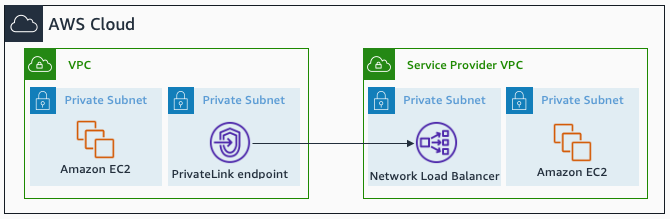
\includegraphics[scale=0.6]{vpc-networking/privatelink}
    \centering
    \label{fig:vpc-privatelink}
\end{figure}

\subsection{Site-to-Site VPN}\label{subsec:site-to-site-vpn}
Connect on-premise VPN to AWS using the public internet (it's encrypted tho).

\begin{figure}[h]
    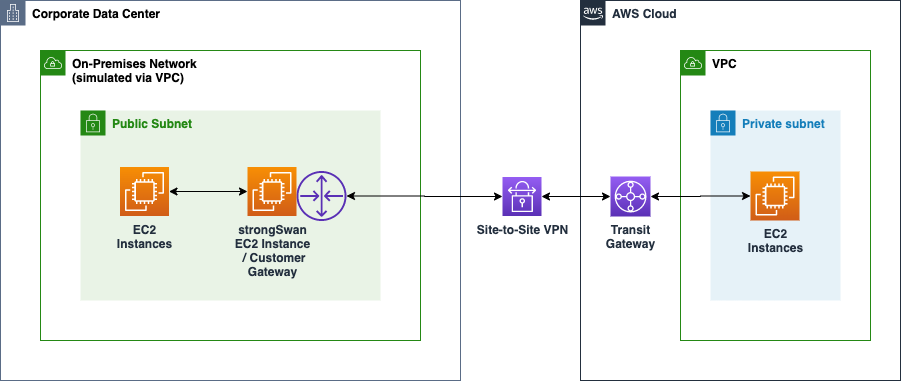
\includegraphics[scale=0.4]{vpc-networking/site-to-site}
    \centering
    \label{fig:vpc-site-to-site}
\end{figure}


\subsection{Direct Connect (DX)}\label{subsec:direct-connect}
Establish physical connection between on-premise and AWS using a private network\@.
Takes month to establish\@.

\subsection{Client VPN}\label{subsec:client-vpn}
Connects from your computer (using OpenVPN) to your private AWS network and on-premise using public internet\@.

\subsection{Transit Gateway}\label{subsec:transit-gateway}
Transitive peering between multiple VPCs and on-premise.
Works with Direct Connect (DX).